% -*- coding: utf-8 -*-
% !TEX encoding = UTF-8 Unicode
% !TEX root =  main.tex

\chapter{Modellbasierte Implementierung der Vektorregelung}
\label{cha:regelungpmsm}

Die Einführung in das Kapitel stellt dem Leser zunächst eine grundlegende Einführung in die Simulationstechniken und dem Anwenderprogramm \product{Simulink} dar.
\product{Simulink} ist ein Programm, welches mit \product{Matlab} gekoppelt ist, in \product{Simulink} kann der Anwender Simulationen durchführen.
Aufgrund der Komplexität von \product{Simulink} soll an dieser Stelle nicht weiter auf die \enquote{Toolboxen} eingeganen werden.
Somit erhalten auch Leser ohne Erfahrungen mit dem Softwarepaket, die zum weiteren Verständnis der Arbeit benötigten Grundkenntnisse.
Der Vorteil bei der Nutzung von \product{Matlab} basiert zum einen darauf, dass die Software etablierter Quasistandard in der Industrie und an Hochschulen ist und zum anderen auf der Benutzerfreundlichkeit bei der Durchführung von Projektarbeiten \autocite{scherf2010}.

\section{Simulation von Systemen}\label{sec:simulation}

Simulationen sind heute unverzichtbar bei der Entwicklung und Optimierung von Systemen und der Erforschung von Zusammenhängen komplexer Systeme und Prozesse \autocite{brychta}.
Die meist umfangreichen Prozesse und Systeme werden dazu in Modellen nachgebildet.
Dieses Verfahren eignet sich gut zur Analyse der Systemeigenschaften.
Dabei können die eingesetzten Simulationsmittel unterschiedlich ausfallen.

\begin{enumerate}
	\item Das System wird maßstäblich oder stark vereinfacht mit den wesentlichen Komponenten aufgebaut.
	\item Das System wird durch ein anderes physikalisches Modell nachgebildet.
	\item Das System wird durch ein mathematisches Modell beschrieben.
\end{enumerate}

Bei umfangreichen Simulationen bietet es sich an, das System in \enquote{Subsysteme} zu unterteilen (s.~h.~Abbildung~\ref{fig:subsysteme}), so dass die Modellierung mit \product{Simulink} übersichtlicher wird.
Der Vorteil gegenüber der konventionellen Modellierung von umfangreichen System, ist es, dass Fehler früher erkannt und einzelne Systeme auf physikalische Richtigkeit geprüft werden können.

\begin{figure}[h!]
	\centering
	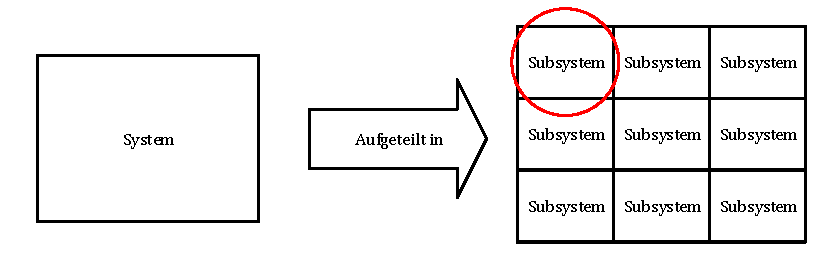
\includegraphics{/simulink/subsysteme.pdf}
	\label{fig:subsysteme}
	\caption{Semantische Darstellung zur Unterteilung eines Systemes in Subsysteme.}
\end{figure}

Das eingekreiste System kann so isoliert und gekapselt beschrieben werden.
Dazu sind die Abhängigkeiten zwischen benachbarten Subsytemen zu erfassen und bei der Kapselung geeignet zu verwerten.
Auch Subsysteme lassen sich in weitere Subsysteme zerlegen (s.~h.~Abbildung~\ref{fig:subsubsysteme}).

\begin{figure}[h!]
	\centering
	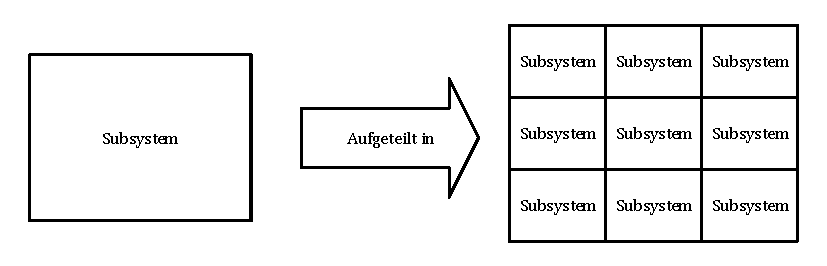
\includegraphics{/simulink/subsubsystem.pdf}
	\label{fig:subsubsysteme}
	\caption{Semantische Darstellung zur Unterteilung eines Subsystems in weitere Subsysteme.}
\end{figure}

Bei der Modellierung sollte auf die Übersichtlichkeit der Systeme geachtet werden.

\section{Einführung in \product{Simulink}}\label{sec:simulink}

\product{Simulink} ist ein grafikorientiertes Softwaretool zur Simulation und Analyse von linearen und nichtlinearen mathematischen Modellen.
\product{Simulink} ist als Unterprogramm von \product{Matlab} implementiert und greift auf dessen numerischen Lösungsalgorithmen zu.
Bei dem Simulationswerkzeug \product{Simulink} handelt es sich um eine \emph{Toolbox} der Programmierumgebung \product{Matlab}.
Sie dient mit ihrer speziell konzipierten Grafikoberfläche der Simulation dynamischer Systeme.
Im Gegensatz zur zeilenorientierten Programmierung mit alphanumerischen Zeichen wird in \product{Simulink} das Systemmodell mittels des \emph{\product{Simulink} Library Browsers} einer nach Funktionen unterteilten Bibliothek entnommen und in das Eingabeoberfläche \enquote{gezogen}.
Dort werden sie per Mausklick sinnvoll miteinander verbunden.
In den meisten Simulationen handelt es sich bei dynamischen Systemen um zeitabhängige, lineare (oder nichtlineare) Vorgänge, die sich auf Basis von Differentialgleichungen beschreiben lassen.
Die Modelle entstehen meistens auf Basis idealisierter Gleichungen.

In der Systemtechnik wird zur Beschreibung häufig eine andere Form bevorzugt (Blockschaltbildern).
Dabei wird versucht, das Verhalten des Systems durch eine grafische Darstellung zu erfassen.
Einzelne Blöcke werden durch gezielte Verbindungen, den Signalflüssen, miteinander verbunden.
Da \product{Simulink} auf dieser Art der Darstellung basiert, ist es offensichtlich, dass sich viele in Form vn Blockschaltbildern vorliegende Systeme unmittelbar in Simulink programmieren und simulieren lassen.
Nach dem Aufbau des Systems im Eingabefenster, müssen die Blöcke parametriert werden.
Anschließend kann die Simulation gestartet werden und das Ergebnis grafisch dargestellt werden.
Die Simulation von \product{Simulink}-Modellen basiert auf iterativen Näherungsverfahren (Runge-Kutta, Adams, usw.).
Das zeitliche Verhalten der simulierten Systeme wird daher in den wenigsten Fällen völlig identisch mit dem Differentialgleichungen erreicht.
Bei korrekter Programmierung und guter Parameterwahl wird es diesem sehr Nahe kommen.

Eine umfassende Hilfe über \product{Simulink} findet man nach Öffnen der \product{Matlab}-Entwicklungsumgebung im \emph{Popup-Menü} \emph{Help}.
Dieses Menü stellt eine Windows-typische Hilfe für die gesamte \product{Matlab}-Produktfamilie zur Verfügung.
Ist \product{Simulink} bereits geöffnet, so führt die Auswahl der Hilfe im \emph{Library Browser} oder im Eingabefenster direkt zur \product{Simulink}-Hilfe.
Darüber hinaus werden in der \product{Simulink}-Hilfe viele Beispiele als lauffähige Programme zur Verfügung gestellt.
Diese findet man in der Hilfe unter \emph{Demos}.

Um mit \product{Simulink} arbeiten zu können, muss zunächst die \product{Matlab}-Entwicklungsumgebung in den Arbeitspeicher geladen werden.
Der Start von \product{Simulink} kann über die Kommandozeile mit \enquote{simulink} erfolgen.

Wie bereits erwähnt, werden (zeitkontinuierliche) dynamische Systeme durch Differentialgleichungen beschrieben, wie z.\ B.\ die normierte Bewegungsgleichung eines gedämpften Schwingers.

\begin{align*}
	\ddot{y}(t) + 2\cdot d\cdot \omega_\x{0}\cdot \dot{y}(t) + \omega_\x{0}^{2} y(t) = u(t)
\end{align*}

Wenn das System durch ein Blockschaltbild beschrieben wird, so betrachtet man nichts anderes, als die Lösung der Differentialgleichung.
In diesem Fall ist \product{Simulink} ein numerischer Differentialgleichungslöser für dieses Projekt.

\subsection{Simulationsbeispiel: Das mathematische Pendel}

Zur Modellbildung und Simulation eines dynamischen Pendels sei zunächst die folgende Abbildung \ref{fig:pendel} gegeben:

\begin{figure}[h]
	\centering
	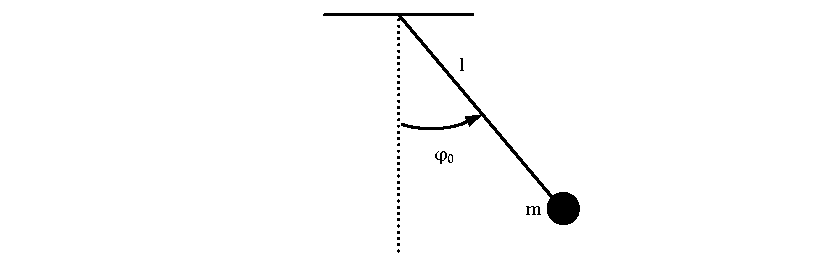
\includegraphics{/regelung/pendel.pdf}
	\label{fig:pendel}
	\caption{Fadenpendel}
\end{figure}

Er gelten folgende Momente:

\begin{center}
	\begin{tabular}{ll}
		\toprule
		Bezeichnung:				&	Mathematisches Modell: \\
		\midrule
		Rückstellmoment				&	$F_\i{Z} = m \cdot g \cdot \si{sin}(\varphi) \label{rueckstellmoment}$ \\
		Beschleunigungsmoment		&	$F_\i{B} = J \cdot \varphi = m \cdot l^{2} \cdot \ddot\varphi\label{beschleunigungsmoment} $ \\
		Reibungsmoment				&	$F_\i{R} = d \cdot l^{2} \cdot \dot\varphi\label{reibungsmoment} $ \\
		Summe aller Kräfte			&	$\sum F = 0 \label{momentengleichgewicht} $ \\
		\bottomrule 
	\end{tabular}
\end{center}
		
Die Bewegung des Pendels wird mit folgenden Werten simuliert:

\begin{center}
	\begin{tabular}{ll}
		\toprule
		Physikalische Bezeichnung:	& Wert: \\
		\midrule
		m		& \SI{2,3}{kg} \\
		d		& \SI{0,2}{Nms} \\
		l		& \SI{1,1}{m} \\
		g		& \SI{9,81}{m/s^2}\\
		$\varphi$ & \SI{40}{^\circ}\\
		\bottomrule
	\end{tabular}
\end{center}
	
Als nächster Schritt werden die physikalischen Systembeschreibungen in einer Gesamtformel zusammengefasst. 

\begin{align}
	\sum M = M_\i{R} + M_\i{B} + M_\i{Reib} = 0
	\label{momentengleichgewichtgesamt} 
\end{align}

\begin{align}
	\sum M = m \cdot g \cdot \si{sin}(\varphi) + J \cdot \varphi = m \cdot l^{2} \cdot \ddot\varphi + d \cdot l^{2} \cdot \dot\varphi = 0
	\label{momentengleichgewichtgesamt2} 
\end{align}

Wird nun die Differentialgleichung \ref{momentengleichgewichtgesamt2} nach der höchsten Ableitung $\ddot\varphi$ umgestellt, ergibt sich:

\begin{align}
	\ddot\varphi = -\dot\varphi \cdot \tfrac{\i{d}}{\i{m}} - \tfrac{\i{g}}{\i{l}} \cdot \si{sin}(\varphi)
	\label{diffgleichung} 
\end{align}

%\begin{figure}[h]
%	\centering
%	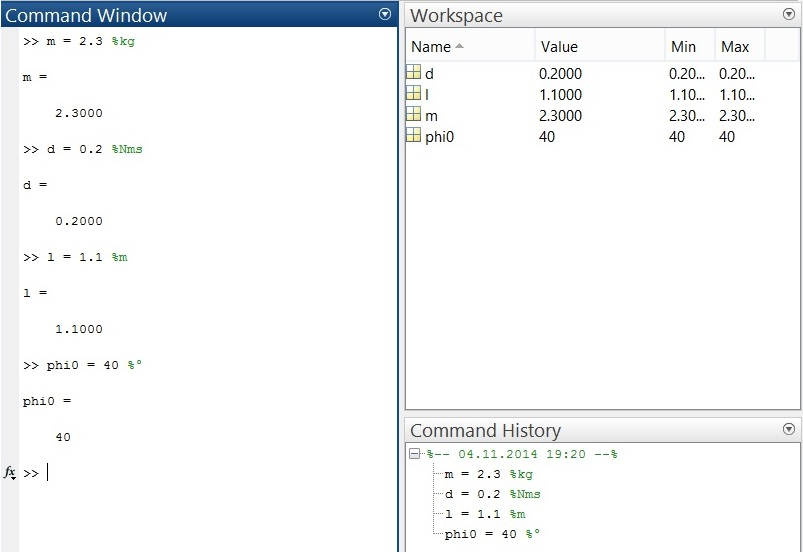
\includegraphics[width=\textwidth]{/regelung/matlab1.jpg}
%	\label{fig:matlab1}
%	\caption{Variablen in \product{Matlab}-Umgebung}
%\end{figure}

Anschließend kann in der \product{Simulink}-Umgebung das Modell entsprechend \ref{momentengleichgewichtgesamt2} aufgebaut werden.

\begin{figure}[h]
	\centering
	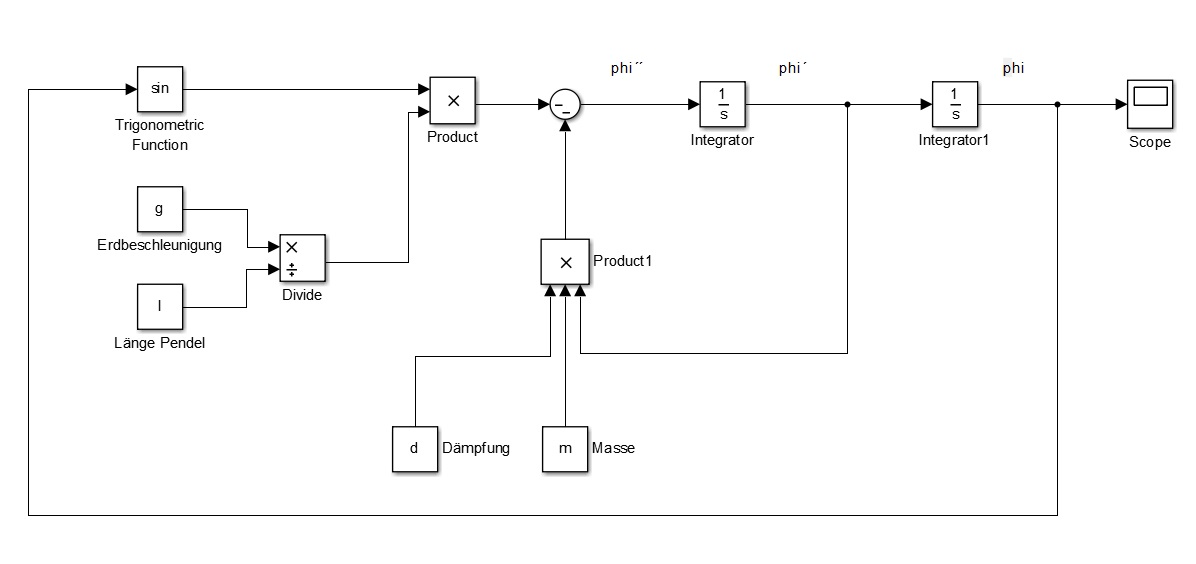
\includegraphics[width=0.8\textwidth]{/regelung/matlab2.jpg}
	\label{fig:matlab2}
	\caption{Modell des mathematischen Pendels in \product{Matlab} \product{Simulink}.}
\end{figure}
\pagebreak
Mit Hilfe dieser Blöcke lassen sich  $\dot{\varphi}$ und $\varphi$ erzeugen.
Die \product{Simulink} Bibliothek bietet eine Vielzahl von mathematischen Operatoren in Form von Blockbildern.
Mit Hilfe dieser Blöcke und der Signalflusspfeile lässt sich die Gleichung in das Simulationsmodell übertragen.
Ist das Modell aufgebaut, werden die Simulationsparameter ausgewählt. 
\product{Simulink} arbeitet numerisch, daher muss ein Integrationsverfahren zur Lösung der DGLs ausgewählt werden. Voreingestellt ist das Dormand-Prince-Verfahren mit variabler Schrittweite.

Diese Methode liefert in den meisten Anwendungen gute Ergebnisse \autocite{scherf2010}.
Zur Verifizierung der Simulationsergebnisse ist es für den Anwender unumgänglich, sich im Vorfeld Gedanken zum erwartenden Ergebnis zu machen.
Im vorliegenden Beispiel sollte der Winkel $\varphi$ eine gedämpfte Schwingung in Abhängigkeit von der Zeit erzeugen.
Das Ergebnis der Simulation erhält der Anwender beim Anwählen des Blockbildes \glqq{Scope}\grqq.
%Hier zeigt sich nach durchgeführter Simulation folgendes Ergebnis:

%\begin{figure}[h!]
%	\centering
%	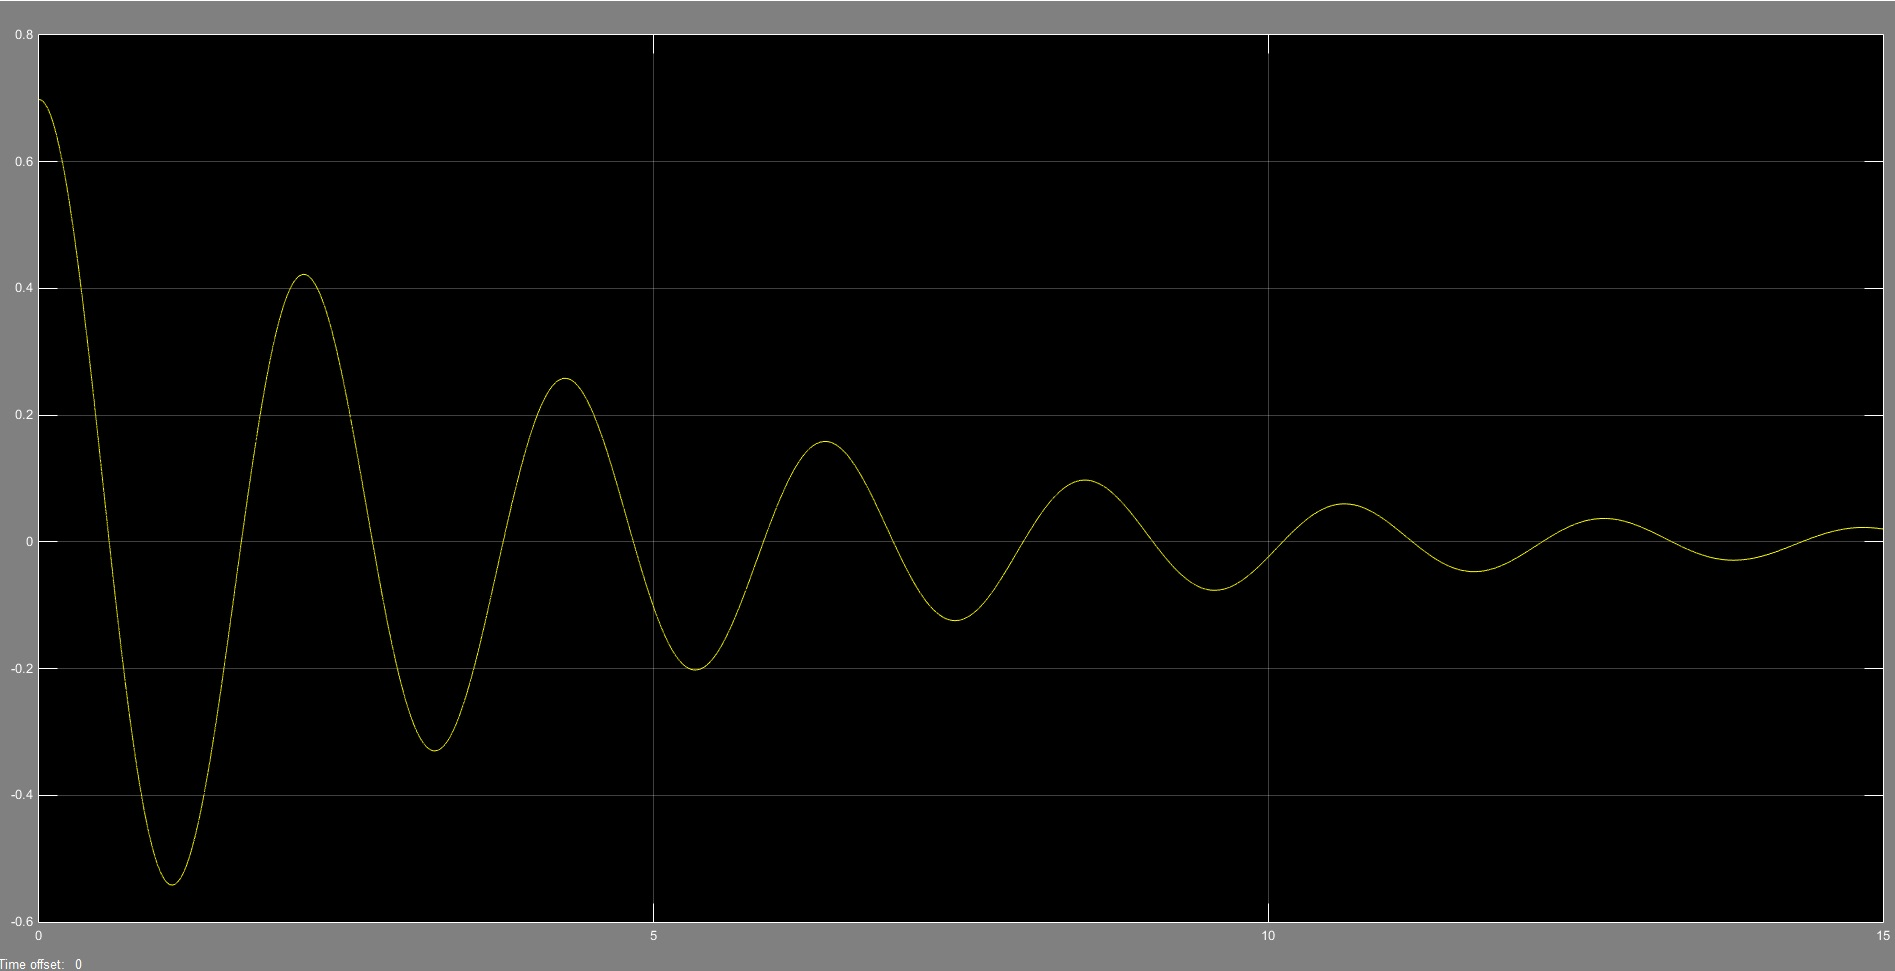
\includegraphics[width=\textwidth]{/regelung/matlab3.jpg}
%	\label{fig:matlab3}
%	\caption{Winkel $\varphi$ des Pendels über die Simulationszeit.}
%\end{figure}

%Wie erwartet, wird eine deutlich gedämpfte Schwingung des simulierten Pendels erkennbar.

\section{Simulationsblöcke}\label{sec:math-model-pmsm}

Dieser Abschnitt zeigt alle Elemente der implementierten Vektorregelung in \product{Matlab} \product{Simulink}.
In Abbildung~\ref{fig:foc-pmsm} ist die gesamte Vektorregelung dargestellt.

\begin{figure}[h!]
	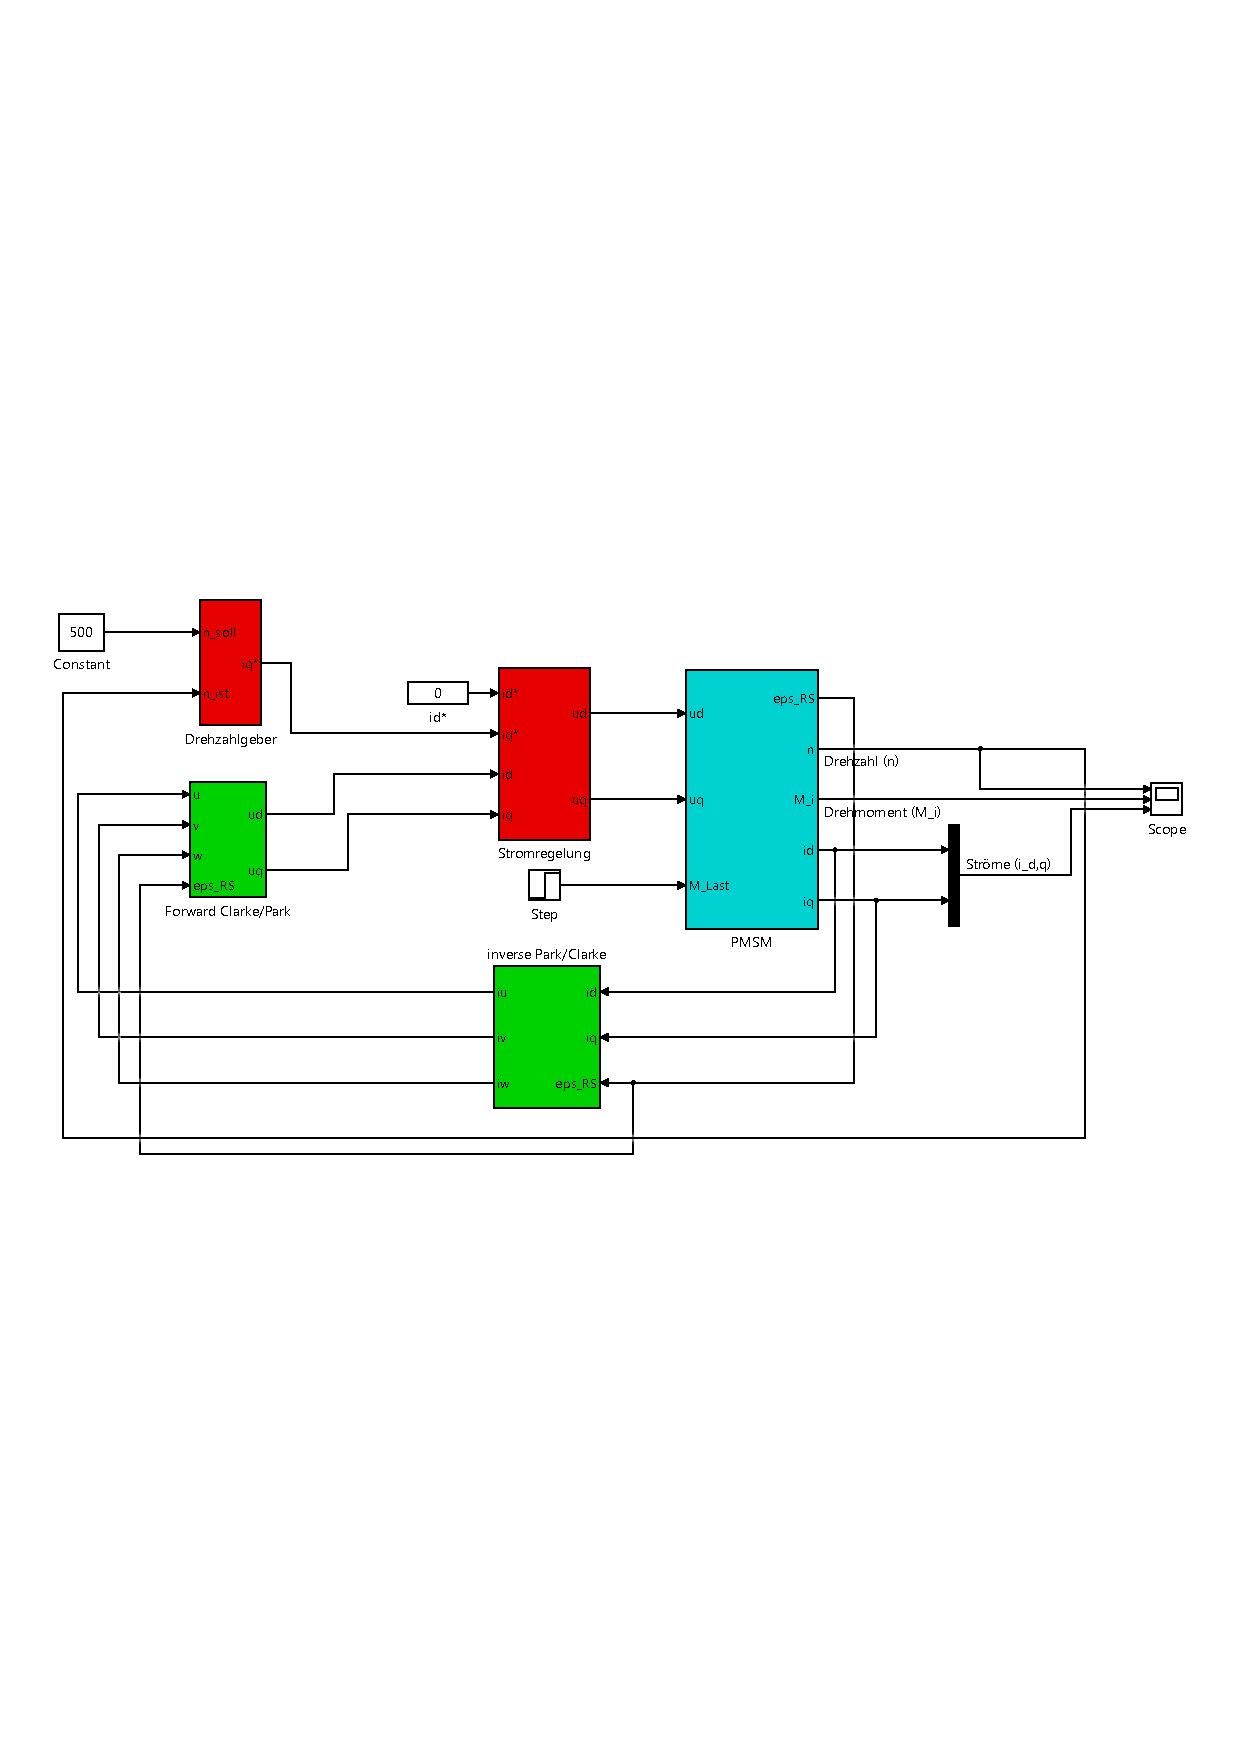
\includegraphics[width=\textwidth]{/simulink/foc-pmsm.pdf}
	\label{fig:foc-pmsm}
	\caption{Darstellung der Simulationsblöcke in \product{Simulink}.}
\end{figure}

Farbig gekennzeichnet sind reglungstechnische Elemente (rot), Transformationen (grün) und das mathematische Maschinenmodell einer anisotropen Synchronmaschine (cyan).
Als \enquote{Step} modelliert ist der Lastsprung, die Drehmoment Anforderung an das System.
Im Folgenden sollen alle Subsysteme entsprechend der Funktionsweise erörtert werden.

\subsection{Transformationsblöcke}

Der Aufbau der Koordinatentransformationen leitet aus Abschnitt \ref{sec:clark} ab. 
Hierbei basiert der Block der $\alpha$-$\beta$-Transformation aus den Zusammenhängen von (\ref{clarkevektor}) und (\ref{clarkematrix}), während die Rücktransformation, die inverse $\alpha$-$\beta$-Transformation mit Hilfe von (\ref{inverseclarkevektornulleinfach}) und (\ref{inverseclarkematrixnulleinfach}) erstellt ist.
Weiterhin orientieren sich die Umsetzungen in \product{Simulink} an den Blockschaltbildern aus \ref{fig:blockbildclarkeparkkomplett} und \ref{fig:blockbildinverseclarkeparkkomplett}.
Um die Koordinatentransformation zu vervollständigen ist die d-q-, oder Park Transformation, von entscheidender Bedeutung.
Der Block für die d-q-Transformation setzt wird mit dem Zusammenhang \ref{parkvektor} und der Matrix \ref{parkmatrix} erstellt. 

\begin{figure}[htb!]
	\centering
	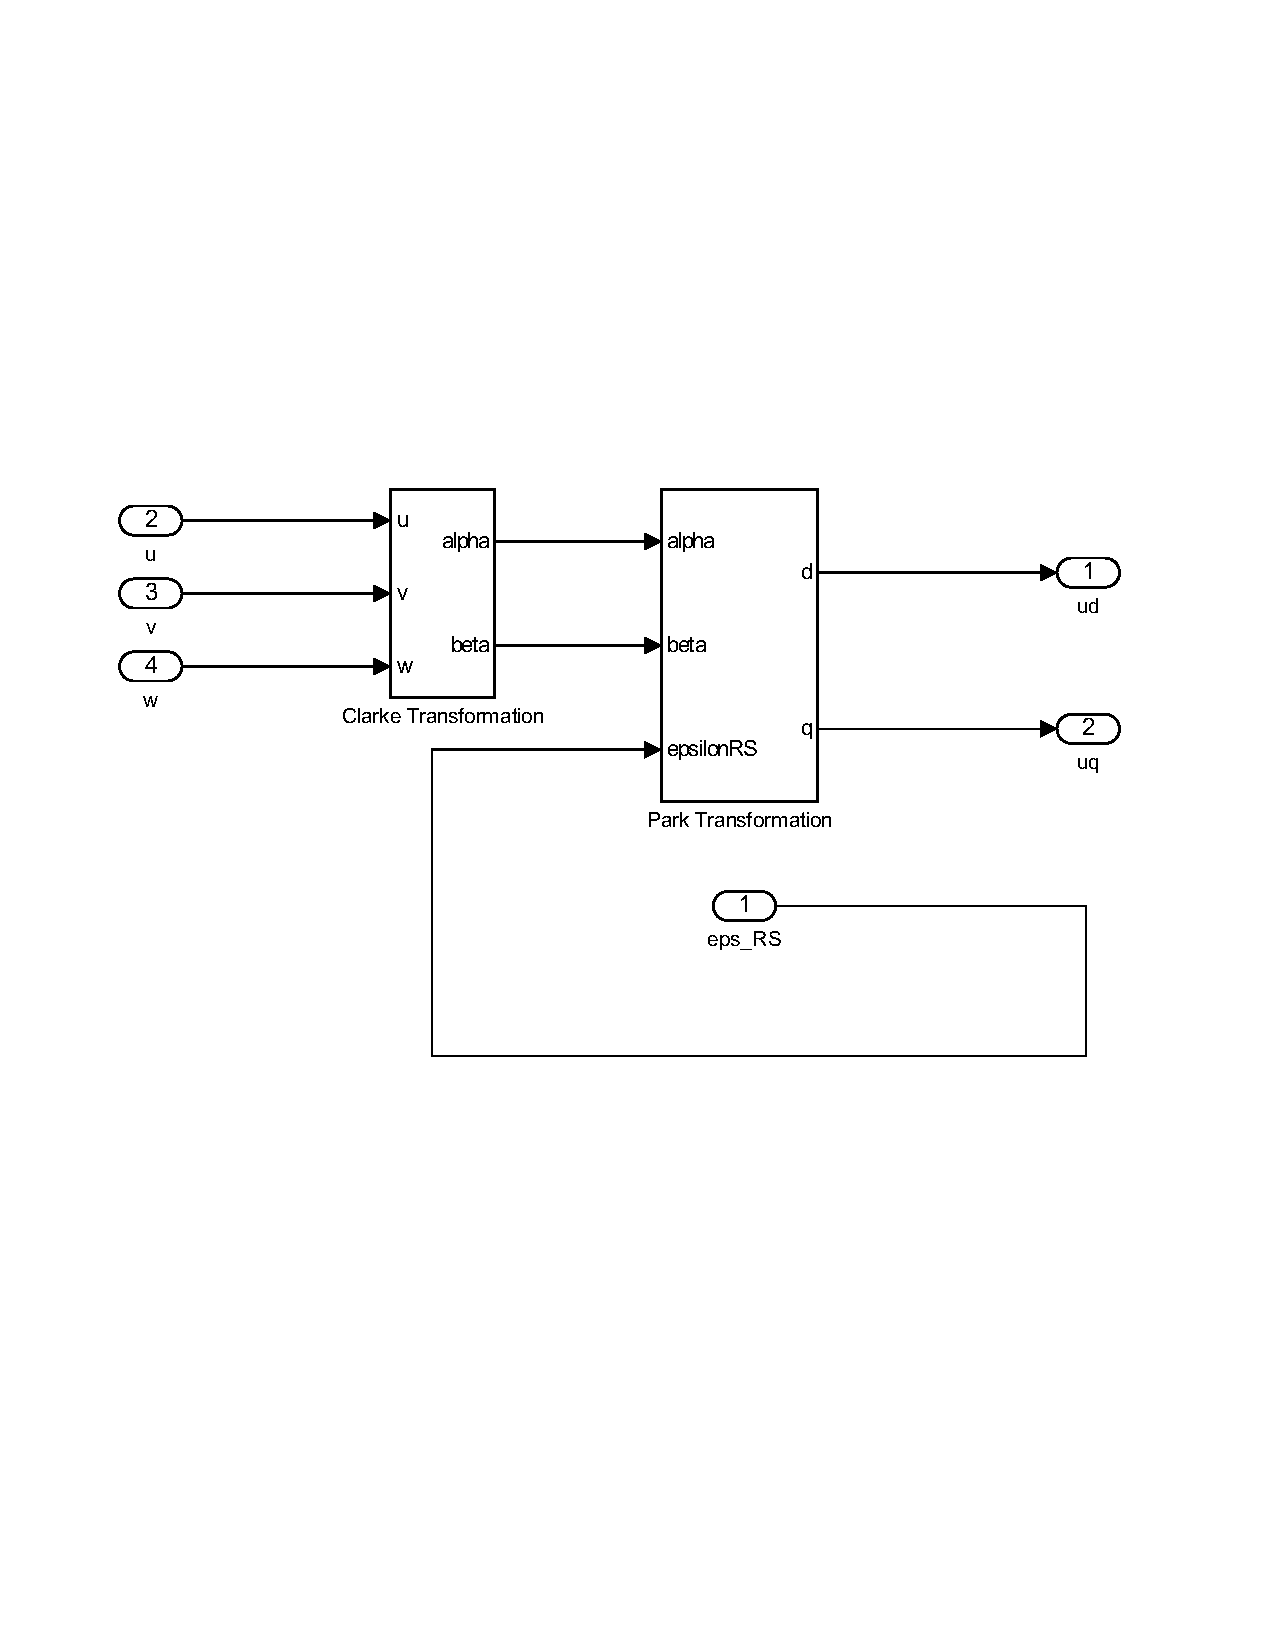
\includegraphics[width=0.8\textwidth]{/simulink/uvw_to_dq.pdf}
	\label{fig:uvw_to_dq}
	\caption{Aufbau Clarke-Park Transformation}
\end{figure}

Die inverse d-q-Transformation ist mit Hilfe der Matritzen \ref{parkvektorinvers} sowie \ref{parkmatrixinvers} aufgebaut.
An dieser Stelle ist es aus übersichtlichkeitsgründen sinnvoll, die Transformationsblöcke als Subsystem zusammenzufassen.
Es ergibt sich für die Clarke-Park Transformation somit ein Block mit drei Eingängen für die drei Wechselgrößen und einem Eingange für $\varepsilon_\i{RS}$, sowie zwei Ausgängen für d- und q-Komponente.
Ebendieses wird auch für die Rücktransformation gemacht. 
Hier ergibt sich ein Subsystem mit drei Eingängen. 
Zwei für d- und q-Größe sowie ebenfalls ein Eingang für $\varepsilon_\i{RS}$.
Es ergeben sich drei Ausgänge für das rückgeführte Dreiphasensystem.

\begin{figure}[htb!]
	\centering
	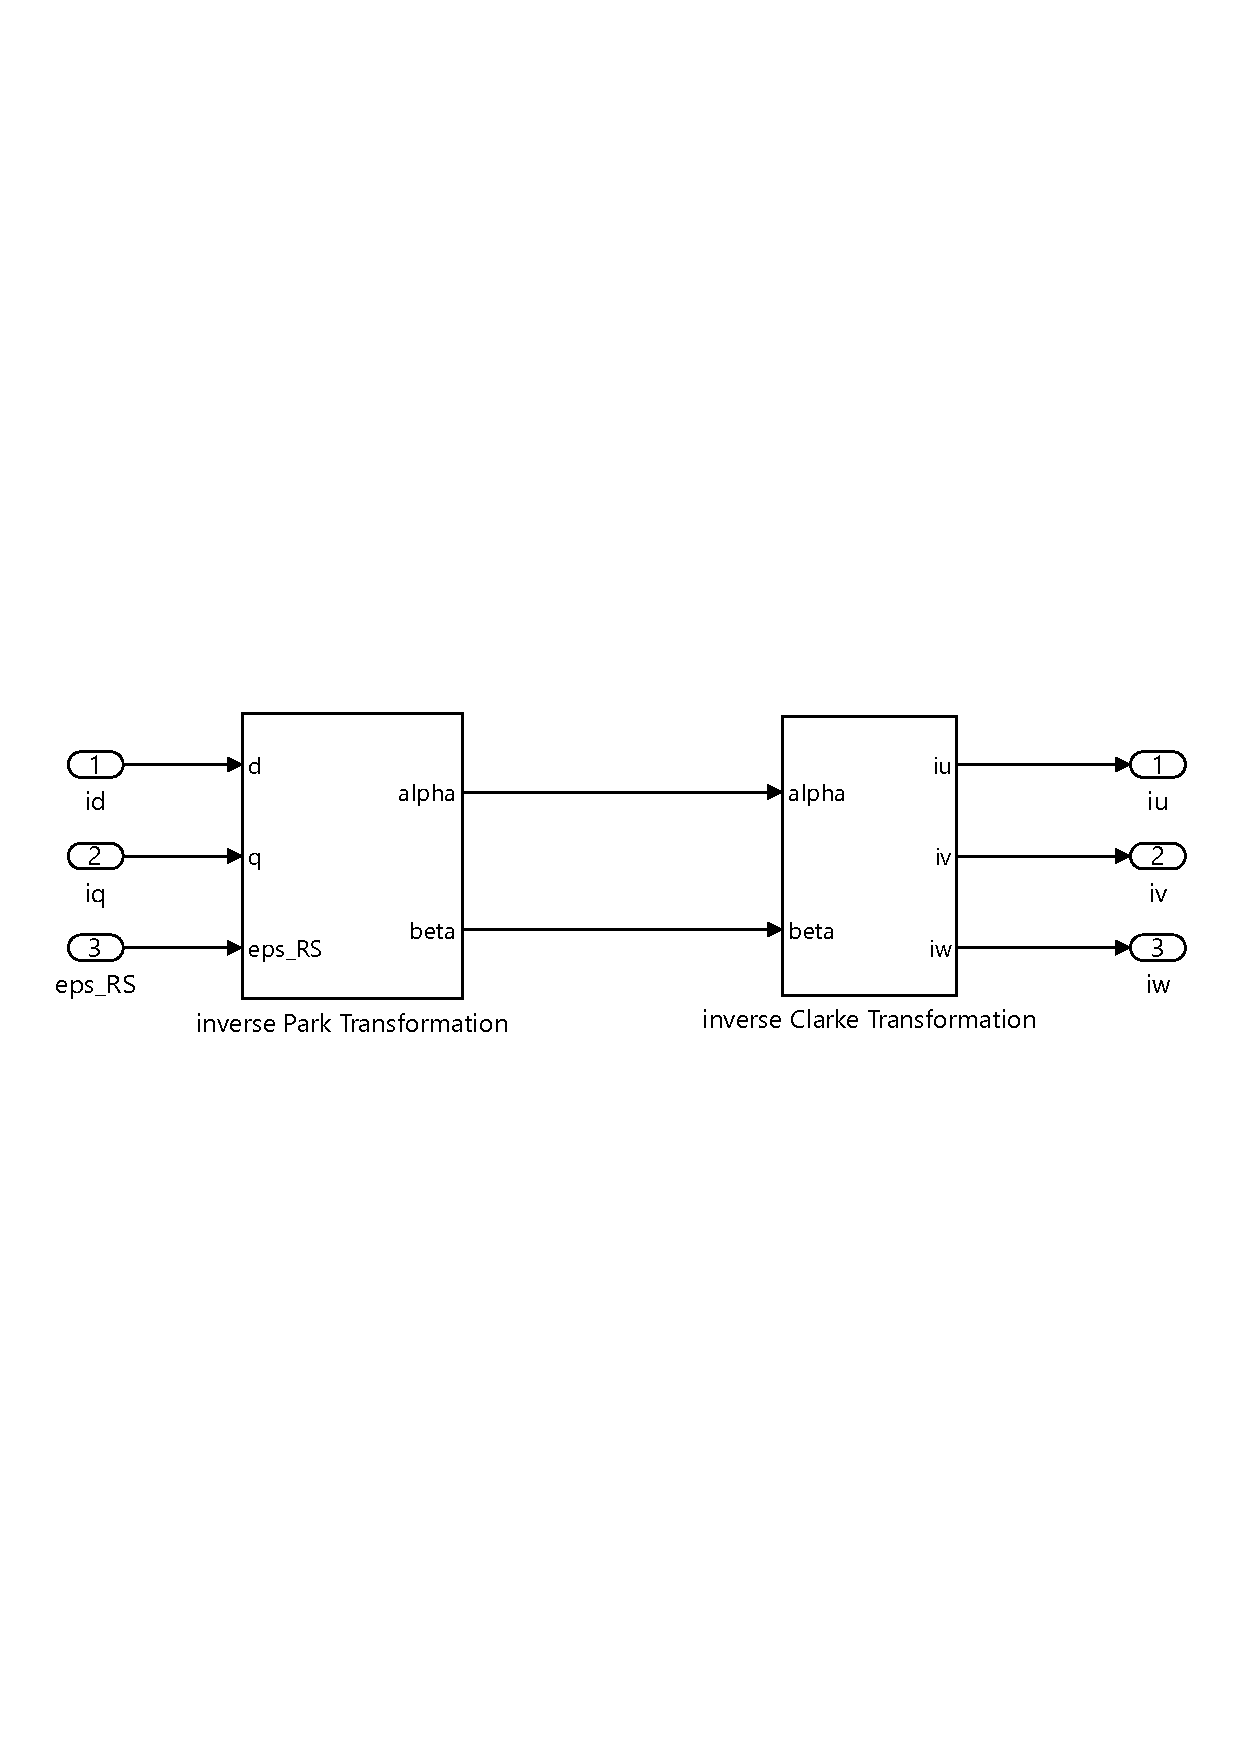
\includegraphics[width=0.8\textwidth]{/simulink/dq_to_uvw.pdf}
	\label{fig:dq_to_uvw}
	\caption{Aufbau inverse Clarke-Park Transformation}
\end{figure}

%\verylongpage

\subsection{Modellierung einer PMSM}

Als Grundlage für die Betrachtung der PMSM gilt der Abschnitt \ref{sec:synchron-dq}.
Die grundlegenden Gleichung dazu sind (\ref{eqn:ud-lin-gleichung}), (\ref{eqn:uq-lin-gleichung}) und (\ref{eqn:mi-lin-gleichung}).
Aus den Gleichungen ergibt sich im \product{Simulink} das Modell.
Das Modell wird in zwei Systeme unterteilt:

\begin{itemize}
	\item Mechanical system
	\item Electrical system
\end{itemize}

\begin{figure}[h!]
	\centering
	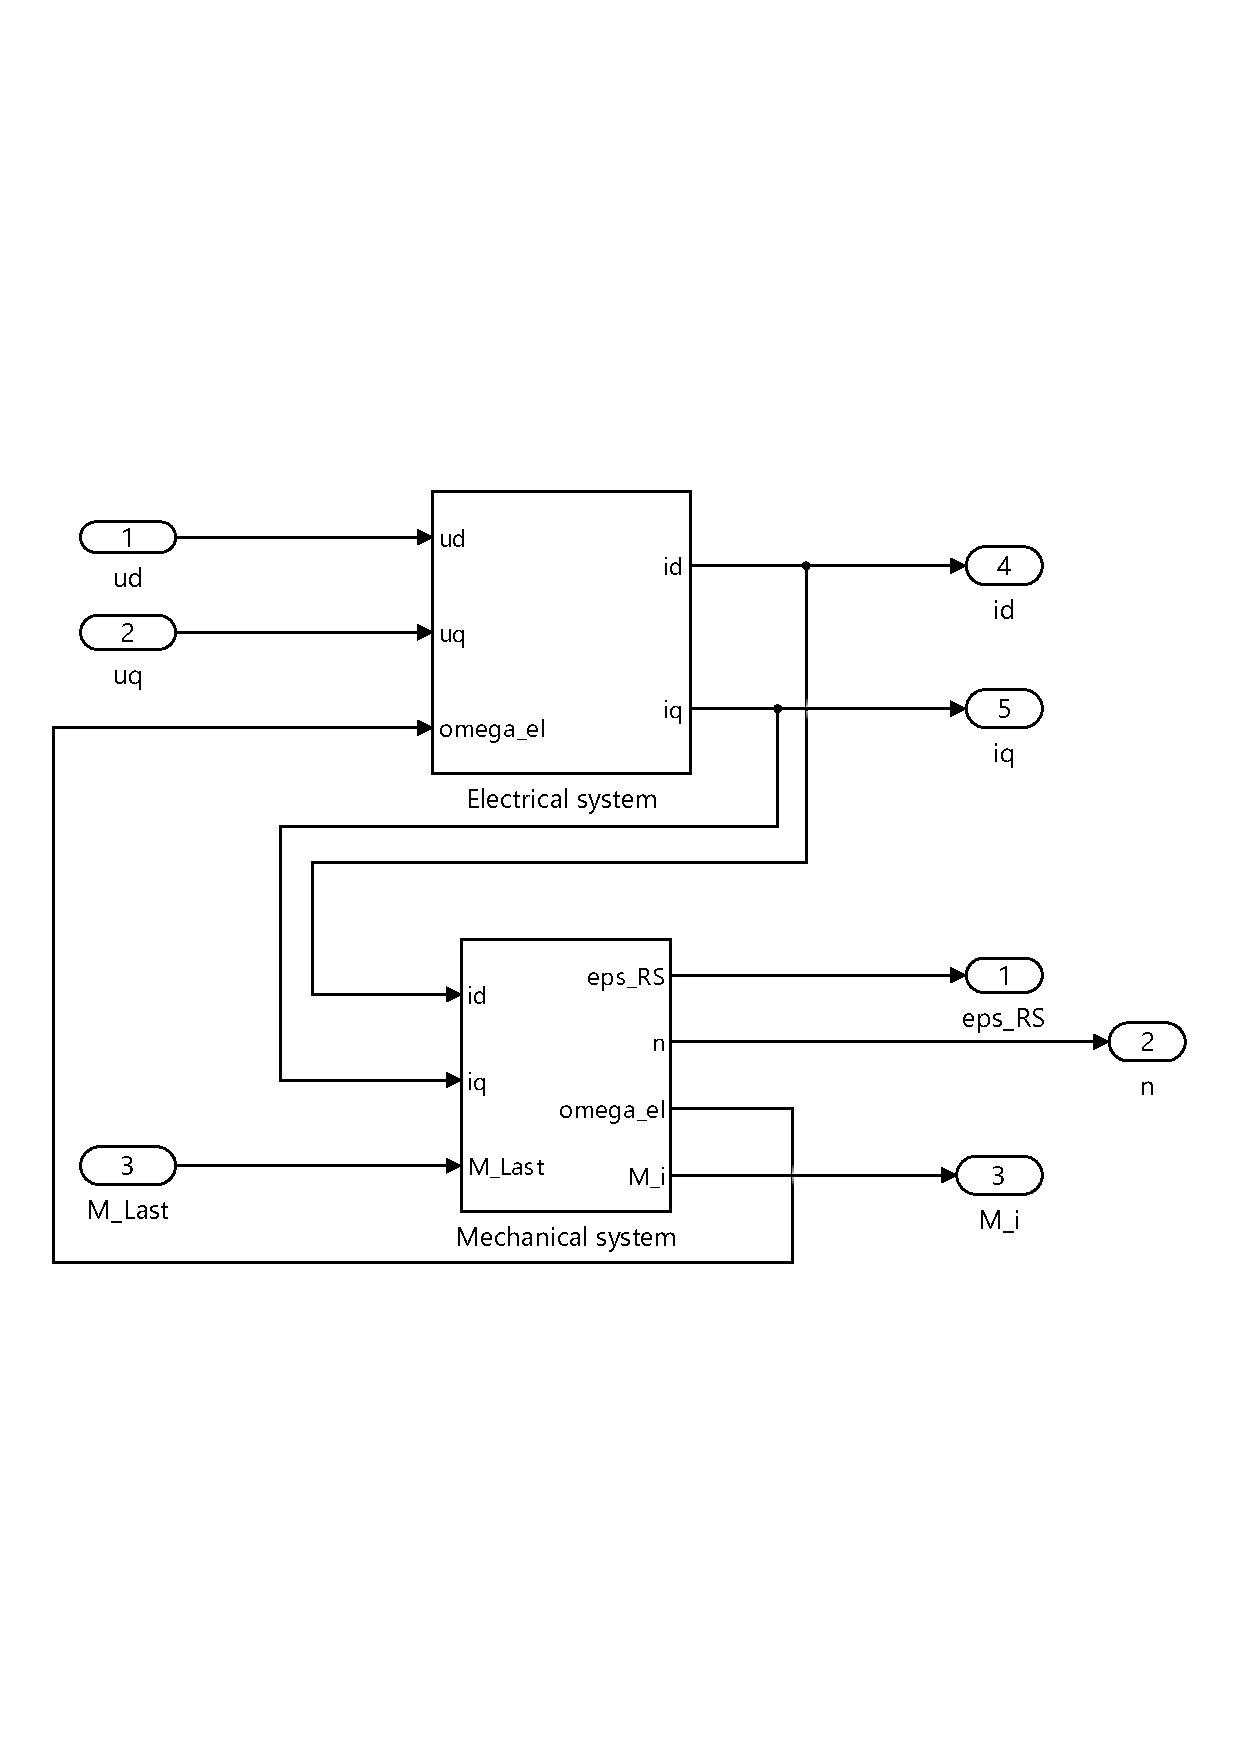
\includegraphics[scale=0.7]{/simulink/pmsm.pdf}
	\label{fig:pmsm}
	\caption{Aufbau des Subsystems: PMSM, mit der Unterteilung in: Electrical system und Mechanical system.}
\end{figure}

Bei dem \enquote{Mechanical system} wird die Differentialgleichung der elektrischen Winkelgeschwindigkeit beschrieben s.~h.~Gleichung~(\ref{eqn:mi-lin-gleichung}).
Das \enquote{Electrical system} beschreibt hingegen die Differentialgleichungen der Ströme und somit die elektrischen Parameter einer PMSM.
Die Überführung der Maschinengleichungen erfolgt dabei dem gleichen Prinzip wie in Abschnitt \ref{cha:regelungpmsm}.
Zunächst wird auf das \enquote{Electrical system} eingegangen, welches in Abbildung \ref{fig:electrical-system} dargestellt ist.
Die dabei modellierten Gleichungen~(\ref{eqn:id_dt}) und (\ref{eqn:iq_dt}) werden entsprechend umgesetzt, dabei entsteht das Modell auf Basis eines vereinfachten Modells (s.~h.~Abschnitt~\ref{sec:synchron-dq}~--~Linearisierte Gleichungen (Spannungsgleichungen im rotorfesten System))~--~das Modell wird ohne Eisenverluste und Sättigungseffekte, wie Wirbelstromverluste, modelliert.
Aus der Bestimmungsgleichung~(\ref{eqn:mi-lin-gleichung}) folgt die elektrische Winkelgeschwindigkeit $\omega_\x{el}$ (s.~h.~Gleichung~(\ref{eqn:dw_dt})).

\subsection{Regelungtechnische Blöcke}

Wie in der Abbildung \ref{fig:foc-pmsm} erkennbar ist, sind reglungstechnische Elemente enthalten.
Zum einen ein Drehzahlgeber (s.~h.~Abbildung~\ref{fig:drehzahl}) und zum anderen die Stromregelung (s.~h.~Abbildung~\ref{fig:stromregelung}).
Wie schon im Abschnitt~\ref{sec:foc} erörtert, regelt die Stromregelung den $i_\x{q}$-Strom~--~damit wird das benötigte Drehmoment realisiert.
Der Drehzahlgeber führt dem System die eingestellte Drehzahl zur Verfügung, so dass die Kombination aus Drehzahlgeber und Stromregelung an einem gemeinsamen Strang ziehen.
Die Stromregelung wird durch zwei einfache PI-Regeler realisiert.
Auch der Drehzahlgeber wird lediglich durch einen PI-Regler realisiert.
Komplexere Regler werden für die feldorientierte Regelung nicht benötigt \autocites{Perassi2006}{kellner2012}.

\begin{figure}[h]
	\centering
	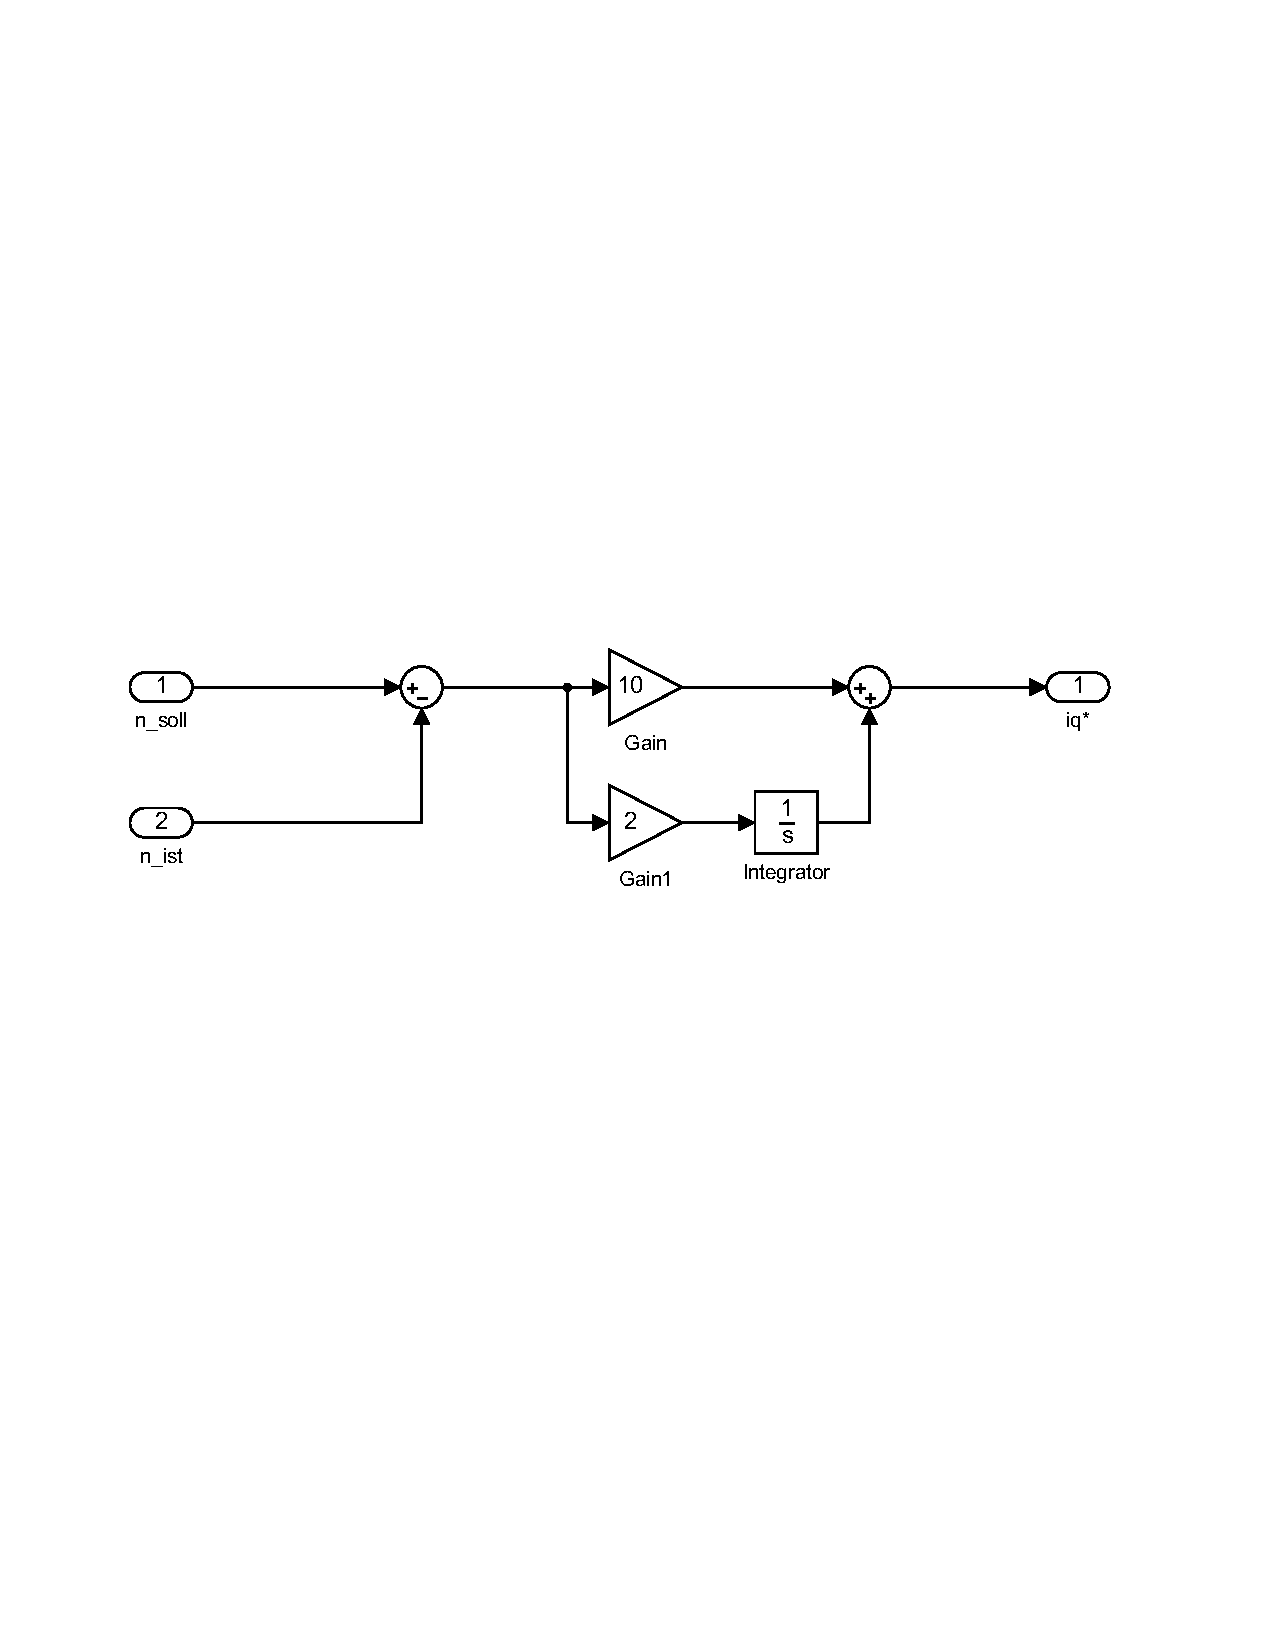
\includegraphics[width=\textwidth]{/simulink/drehzahl.pdf}
	\label{fig:drehzahl}
	\caption{Aufbau der Drehzahlregelung.}
\end{figure}

\begin{figure}[h]
	\centering
	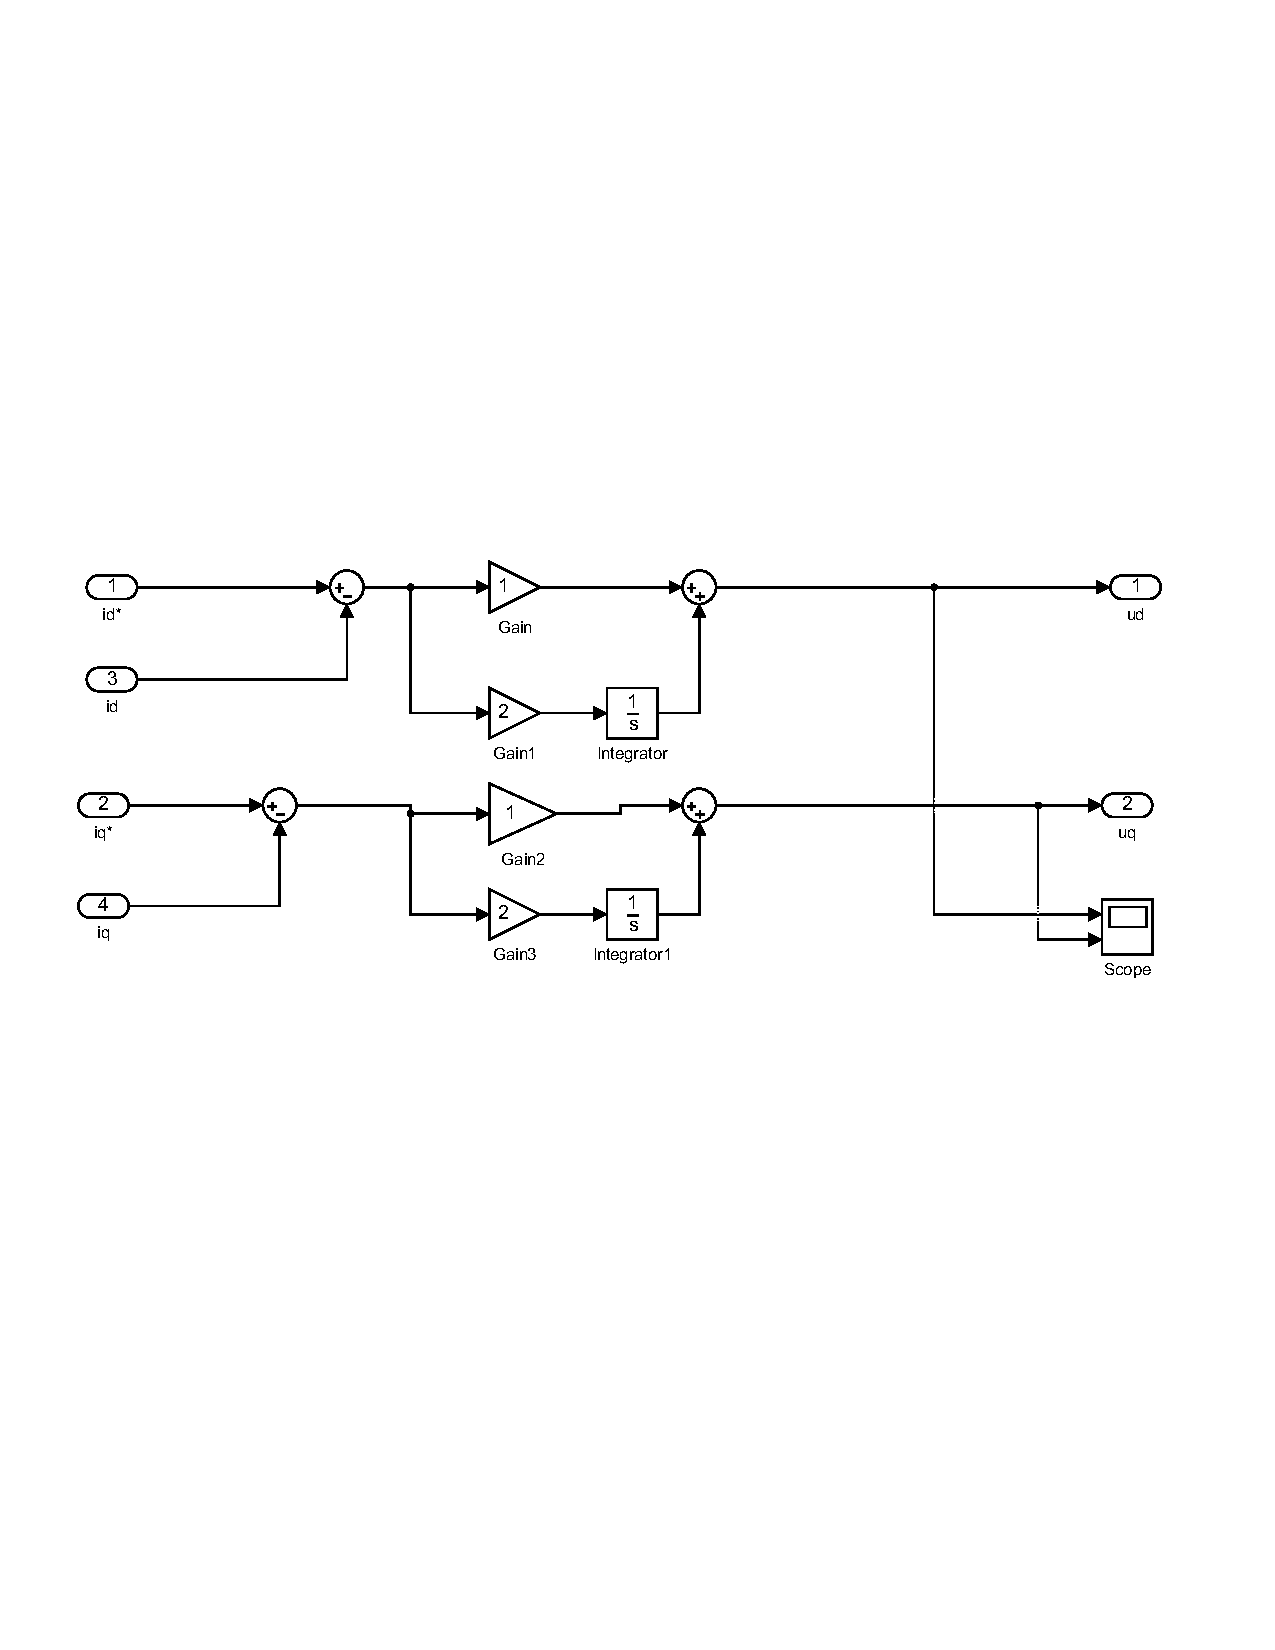
\includegraphics[width=\textwidth]{/simulink/stromregelung.pdf}
	\label{fig:stromregelung}
	\caption{Aufbau der Stromregelung.}
\end{figure}

Der PI-Block aus der \enquote{\product{Simulink} $\rightarrow$ Modeling $\rightarrow$ Block Libraries $\rightarrow$ Continous} Bibliothek ist standardmäßig als \enquote{Continuos-time} Block konfiguriert.
Hinter dem Block stecken ähnlich wie in Abbildung \ref{fig:foc-dc-ac} veranschaulicht eine einfache mathematische Gleichung.
Zudem sei gesagt, dass eine Parallele Regelstruktur angenommen wird:

\begin{align}
	P + I\cdot\frac{1}{s}
\end{align}

Dabei steht $P$ für die Verstärkung des Reglers und $I$ für die Verstärkung des Integralen Anteils.

\begin{quote}
	\enquote{[\ldots] Specify the proportional gain P. [\ldots] Specify the integral gain I. [\ldots] (Mathworks Help -- PID Controller, Discrete PID Controller. In: \product{Simulink} $\rightarrow$ Modeling $\rightarrow$ Block Libraries $\rightarrow$ Continous)}
\end{quote}

%%% Local Variables: 
%%% mode: latex
%%% TeX-master: "main"
%%% TeX-open-quote: "\\enquote{"
%%% TeX-close-quote: "}"
%%% LaTeX-csquotes-open-quote: "\\enquote{"
%%% LaTeX-csquotes-close-quote: "}"
%%% End: 
